%%%%%%%%%%%%%%%%%%%%%%%%%
\section{تحلیل الگوریتم‌ها}
%%%%%%%%%%%%%%%%%%%%%%%%%

\begin{frame}{‌تحلیل الگوریتم‌ها}
\begin{itemize}\itemr
\item[-]
آنالیز الگوریتم یا تحلیل الگوریتم
\fn{1}{algorithm analysis}
به معنای پیش بینی منابع مورد نیاز برای اجرای یک الگوریتم است.
منابع مورد نیاز شامل زمان محاسبات، میزان حافظه، پهنای باند ارتباطی و مصرف انرژی می‌شود.
\item[-]
معمولا برای یک مسئله الگوریتم‌های متعددی وجود دارند که هر یک می‌تواند از لحاظ تعدادی از معیارهای ارزیابی بهینه باشد.
\item[-]
برای تحلیل الگوریتم از یک مدل محاسباتی استفاده می‌کنیم. در اینجا از مدل محاسباتی ماشین دسترسی تصادفی
\fn{2}{random-access machine (RAM)}
استفاده می‌کنیم. در این مدل محاسباتی فرض می‌کنیم زمان مورد نیاز برای اجرای دستورات و دسترسی به حافظه، ثابت و به میزانی معین است.
\item[-]
دستورات معمول در این مدل محاسباتی شامل دستورات محاسباتی ریاضی (مانند جمع و تفریق و ضرب و تقسیم و باقیمانده و کف و سقف)، دستورات جابجایی داده (مانند ذخیره، بارگیری و کپی) و دستورات کنترلی (مانند شرطی و انشعابی و فراخوانی تابع) می‌شوند.
\end{itemize}
\end{frame}


\begin{frame}{‌تحلیل الگوریتم‌ها}
\begin{itemize}\itemr
\item[-]
عملیات محاسبه توان جزء دستورات اصلی مدل محاسباتی رم به حساب نمی‌آید، اما بسیاری از ماشین‌ها با عملیات انتقال بیت‌ها در زمان ثابت می‌توانند اعداد توانی را محاسبه کنند.
\item[-]
همچنین در این مدل، سلسله مراتب حافظه مانند حافظه نهان
\fn{1}{cache memory}
که در کامپیوترهای واقعی پیاده سازی شده است، وجود ندارد.
\item[-]
مدل محاسباتی ماشین دسترسی تصادفی یک مدل ساده همانند ماشین تورینگ است که در آن دسترسی تصادفی به حافظه وجود دارد و عملیات ساده تعریف شده‌اند.
\end{itemize}
\end{frame}

\begin{frame}{‌تحلیل الگوریتم‌ها}
\begin{itemize}\itemr
\item[-]
تحلیل الگوریتم‌ها به منظور محاسبهٔ زمان اجرا و میزان حافظه مورد نیاز الگوریتم‌ها به کار می‌رود.
\item[-]
زمان اجرا و میزان حافظهٔ مورد نیاز یک الگوریتم به ازای ورودی‌های مختلف متفاوت است و این مقادیر بر اساس اندازهٔ ورودی الگوریتم محاسبه می‌شوند.
\item[-]
زمان اجرا و میزان حافظه مورد نیاز، معیارهایی برای سنجش کارایی الگوریتم‌ها هستند.
\item[-]
در این قسمت در مورد روش‌های مختلف تحلیل الگوریتم صحبت خواهیم کرد.
\item[-]
عوامل زیادی در زمان اجرای یک الگوریتم تأثیر می‌گذارند که از آن جمله می‌توان به سرعت پردازنده، کامپایلر استفاده شده برای پیاده سازی الگوریتم، اندازهٔ ورودی الگوریتم و همچنین ساختار الگوریتم اشاره کرد.
\end{itemize}
\end{frame}


\begin{frame}{‌تحلیل الگوریتم‌ها}
\begin{itemize}\itemr
\item[-]
برخی از این عوامل در کنترل برنامه نویس نیستند. برای مثال سرعت پردازنده عاملی است تأثیر گذار در سرعت اجرا که با پیشرفت صنعت سخت افزار بهبود می‌یابد و در کنترل برنامه نویس نیست. اما ساختار الگوریتم عاملی است که توسط طراح الگوریتم کنترل می‌شود و نقش مهمی در سرعت اجرا دارد.
\item[-]
صرف نظر از عوامل فیزیکی، می‌توان سرعت اجرای برنامه را تابعی از اندازهٔ ورودی الگوریتم تعریف کرد که تعداد گام‌های لازم برای محاسبهٔ خروجی را بر اساس اندازه ورودی الگوریتم بیان می‌کند.
\item[-]
تعداد گام‌های یک الگوریتم برای محاسبه یک مسئله به ساختار آن الگوریتم بستگی دارد و تابعی از اندازهٔ ورودی مسئله است.
\item[-]
البته غیر از اندازهٔ ورودی، ساختار ورودی هم بر سرعت اجرای برنامه تأثیر گذار است. بنابراین سرعت اجرای برنامه را معمولاً در بهترین حالت (یعنی حالتی که ساختار ورودی به گونه‌ای است که الگوریتم کمترین زمان را برای اجرا بر روی یک ورودی با اندازه معین نیاز دارد) و بدترین حالت محاسبه می‌کنیم. همچنین می‌توان زمان اجرای برنامه را در حالت میانگین به دست آورد.
\end{itemize}
\end{frame}


\begin{frame}{‌‌تحلیل الگوریتم‌ها}
\begin{itemize}\itemr
\item[-]
یک روش برای تحلیل زمان مورد نیاز برای اجرای الگوریتم مرتب‌سازی، اجرای آن الگوریتم بر روی یک کامپیوتر و اندازه‌گیری زمان اجرا آن است.
\item[-]
اما این اندازه‌گیری به ماشین مورد استفاده و کامپایلر و زبان برنامه نویسی مورد استفاده و اجرای برنامه‌های دیگر برروی آن ماشین بستگی دارد. نوع پیاده سازی و اندازهٔ ورودی نیز دو عامل دیگر در سرعت اجرای برنامهٔ مرتب سازی است.
\item[-]
روش دیگر برای محاسبه زمان اجرای الگوریتم مرتب‌سازی، تحلیل خود الگوریتم است. در این روش محاسبه می‌کنیم هر دستور در برنامه چندبار اجرا می‌شوند. سپس فرمولی به دست آوریم که نشان دهندهٔ زمان اجرای برنامه است. این فرمول به اندازهٔ ورودی الگوریتم بستگی پیدا می‌کند ولی عوامل محیطی مانند سرعت پردازنده در آن نادیده گرفته می‌شود. از این روش می‌توان برای مقایسهٔ الگوریتم‌ها استفاده کرد.
\end{itemize}
\end{frame}


\begin{frame}{‌تحلیل الگوریتم‌ها}
\begin{itemize}\itemr
\item[-]
اندازهٔ ورودی
\fn{1}{input size}
در بسیاری از مسائل مانند مسئله مرتب‌سازی تعداد عناصر تشکیل دهندهٔ ورودی است.
در مسئله مرتب‌سازی اندازه ورودی در واقع تعداد عناصر آرایهٔ ورودی برای مرتب‌سازی است.
\item[-]
در برخی از مسائل اندازهٔ ورودی در واقع تعداد بیت عدد صحیح ورودی است. برای مثال اندازهٔ ورودی مسئله تجزیهٔ یک عدد به عوامل اول، خود عدد ورودی است.
\item[-]
در برخی مسائل تعداد ورودی‌ها بیش از یک پارامتر است، بنابراین اندازهٔ ورودی به بیش از یک پارامتر بستگی پیدا می‌کند. برای مثال در الگوریتم پیدا کردن کوتاه‌ترین مسیر در یک گراف، اندازهٔ ورودی تعداد رئوس و تعداد یال‌ها است.
\end{itemize}
\end{frame}


\begin{frame}{‌‌تحلیل الگوریتم‌ها}
\begin{itemize}\itemr
\item[-]
زمان اجرای
\fn{1}{execution time}
یک الگوریتم وابسته به تعداد دستورات اجرا شده و تعداد دسترسی‌ها به حافظه است.
در هنگام محاسبات برای تحلیل الگوریتم فرض می‌کنیم برای اجرای یک دستور در برنامه به یک زمان ثابت نیاز داریم.
یک دستور در اجراهای متفاوت ممکن است زمان اجرای متفاوتی داشته باشد ولی فرض می‌کنیم خط
\m{k}
ام برنامه، در زمان
\m{c_k}
اجرا شود.
\item[-]
کل زمان اجرای یک برنامه، مجموع زمان اجرای همهٔ دستورات آن است. دستوری که m بار در کل برنامه تکرار می‌شود و در زمان
\m{c_k}
 اجرا می‌شود، در کل به
\m{m c_k}
واحد زمان برای اجرا نیاز دارد.
\item[-]
معمولاً زمان اجرای یک الگوریتم با ورودی
\m{n}
را با
\m{T(n)}
نشان می‌دهیم.
\end{itemize}
\end{frame}


\begin{frame}{‌تحلیل الگوریتم‌ مرتب‌سازی درجی}
\begin{itemize}\itemr
\item[-]
 الگوریتم مرتب‌سازی درجی را یک بار دیگر در نظر می‌گیریم.
\begin{algorithm}[H]\alglr
  \caption{Insertion Sort} 
  \begin{algorithmic}[1]
    \Func{Insertion-Sort}{A, n}
    \newline\LeftComment{A is an array of n elements}
      \For{i = 2 \To n}
        \State key = A[i]
        \State j = i - 1
        \While{ j > 0 and A[j] > key }
          \State A[j+1] = A[j]
          \State j = j-1
        \EndWhile
        \State A[j+1] = key
      \EndFor
  \end{algorithmic}
  \label{alg:insertion-sort}
\end{algorithm}
\end{itemize}
\end{frame}


\begin{frame}{‌تحلیل الگوریتم‌ مرتب‌سازی درجی}
\begin{itemize}\itemr
\item[-]
برای محاسبه زمان اجرای الگوریتم مرتب‌سازی درجی، ابتدا تعداد تکرار هر یک از خط‌های برنامه را می‌شماریم.
\item[-]
در این برنامه خط ۱ تعداد n بار و خطوط ۲ و ۳ و ۷ هر یک
\m{n-1}
 بار تکرار می‌شوند.
\item[-]
تعداد تکرار خطوط ۴ و ۵ و ۶ به تعداد تکرار حلقه بستگی دارد.
\item[-]
زمان اجرای یک الگوریتم علاوه بر اندازه ورودی به ساختار ورودی نیز بستگی دارد. در الگوریتم مرتب‌سازی مسلماً مرتب‌سازی یک آرایهٔ مرتب شده از مرتب‌سازی یک آرایهٔ مرتب نشده سریع‌تر انجام می‌شود.
\end{itemize}
\end{frame}


\begin{frame}{‌تحلیل الگوریتم‌ مرتب‌سازی درجی}
\begin{itemize}\itemr
\item[-]
زمان اجرای یک الگوریتم را معمولا در بهترین حالت و بدترین حالت محاسبه می‌کنیم. در بهترین حالت آرایهٔ ورودی الگوریتم مرتب شده است. بنابراین در بهترین حالت در هر بار اجرای خط ۴ ، برنامه از حلقه
\code{while}
خارج می‌شود و بنابراین خط ۴ تعداد
\m{n-1}
بار اجرا می‌شود و خطوط ۵ و ۶ اجرا نمی‌شوند.
\item[-]
زمان کل اجرای برنامه را می‌توانیم به صورت زیر بنویسیم.
\begin{align*}
\m{T(n)} & \m{= c_1 n + c_2(n-1) + c_3(n-1) + c_4(n-1) + c_7(n-1)}\\
& \m{= (c_1 + c_2 + c_3 + c_4 + c_7)n - (c_2 + c_3 + c_4 + c_7)}
\end{align*}
\item[-]
زمان اجرای این الگوریتم در بهترین حالت را می‌توانیم به صورت
\m{an + b}
بنویسیم به ازای اعداد ثابت a و b و اندازه ورودی n .
بنابراین زمان اجرا در این حالت یک تابع خطی
\fn{1}{linear function}
از n است.
\end{itemize}
\end{frame}


\begin{frame}{‌تحلیل الگوریتم‌ مرتب‌سازی درجی}
\begin{itemize}\itemr
\item[-]
حال زمان اجرای الگوریتم مرتب سازی درجی را در بدترین حالت محاسبه می‌کنیم. در بدترین حالت آرایهٔ ورودی به صورت معکوس مرتب شده است و بنابراین هر یک از عناصر آرایه نیاز به بیشترین تعداد جابجایی دارد.
\item[-]
در حلقهٔ
\code{while}
هر یک از عناصر
\m{A[i]}
باید با همهٔ عناصر
\m{A[1 : i-1]}
مقایسه شود بنابراین حلقه باید تعداد i بار به ازای
\m{2,3,...,n}
تکرار شود.
\item[-]
پس به طور کل خط ۴ باید به تعداد زیر تکرار شود.
\begin{align*}
\m{\sum_{i = 2}^{n} i = \Big(\sum_{i = 1}^{n} i \Big) - 1 = \frac{n(n+1)}{2} - 1}
\end{align*}
\end{itemize}
\end{frame}


\begin{frame}{‌تحلیل الگوریتم‌ مرتب‌سازی درجی}
\begin{itemize}\itemr
\item[-]
هر یک از خطوط ۵ و ۶ الگوریتم به ازای
\m{i = 2,3,...,n}
تعداد
\m{i-1}
بار تکرار می‌شود.
\item[-]
بنابراین برای خطوط ۵ و ۶ تعداد تکرار برابر است با :
\begin{align*}
\m{\sum_{i = 2}^{n} (i-1) = \sum_{i = 1}^{n-1} i  = \Big(\sum_{i = 1}^{n} i \Big) - n = \frac{n(n+1)}{2}-n =  \frac{n(n-1)}{2}}
\end{align*}
\end{itemize}
\end{frame}


\begin{frame}{‌تحلیل الگوریتم‌ مرتب سازی درجی}
\begin{itemize}\itemr
\item[-]
زمان اجرای برنامه در بدترین حالت را می‌توانیم به صورت زیر محاسبه کنیم.
\begin{align*}
\m{T(n)} &\m{= c_1n + c_2(n-1) + c_3(n-1) + c_4(\frac{n(n+1)}{2} - 1)}\\
&\m{~+~c_5(\frac{n(n-1)}{2}) + c_6(\frac{n(n-1)}{2}) + c_7(n-1)}\\
&\m{= (\frac{c_4 + c_5 + c_6}{2})n^2 + (c_1 + c_2 + c_3 + \frac{c_4 - c_5 - c_6}{2} + c_7)n} \\
& \m{~-~(c_2 + c_3 + c_4 + c_7)}
\end{align*}
\end{itemize}
\end{frame}


\begin{frame}{‌تحلیل الگوریتم‌ مرتب‌سازی درجی}
\begin{itemize}\itemr
\item[-]
بنابراین زمان اجرای الگوریتم مرتب سازی درجی در بدترین حالت را می‌توانیم به صورت
\m{an^2+bn+c}
بنویسیم به طوری که a و b و c اعداد ثابت و n ورودی برنامه است. پس زمان اجرای الگوریتم در بدترین حالت یک تابع مربعی
\fn{1}{quadratic function}
یا تابع درجه دوم از n است.
\end{itemize}
\end{frame}


\begin{frame}{‌تحلیل الگوریتم‌ مرتب‌سازی درجی}
\begin{itemize}\itemr
\item[-]
در حالت کلی از آنجایی که تعداد تکرارها در حلقه
\code{while}
مشخص نیست، زمان اجرای الگوریتم را می‌توانیم به صورت زیر بنویسیم که در آن
\m{t_i}
تعداد متغیر تکرارهای حلقه
\code{while}
است.
\begin{align*}
\m{T(n)} &\m{= c_1n + c_2(n-1) + c_3(n-1) + c_4 \sum_{i = 2}^{n} t_i }\\
&\m{+  c_5 \sum_{i = 2}^{n} (t_i-1) +  c_6 \sum_{i = 2}^{n} (t_i-1) + c_7(n-1)}
\end{align*}
\end{itemize}
\end{frame}


\begin{frame}{‌تحلیل الگوریتم‌ مرتب‌سازی درجی}
\begin{itemize}\itemr
\item[-]
معمولاً در تحلیل  الگوریتم‌ها، بدترین حالت
\fn{1}{worst case}
زمان اجرا را محاسبه می‌کنیم.
\item[-]
دلیل این امر آن است که زمان اجرا در بدترین حالت در واقع یک کران بالا
\fn{2}{upper bound}
برای زمان اجرا است و الگوریتم نمی‌تواند به زمانی بیشتر از آن نیاز داشته باشد. پس می‌توانیم تضمین کنیم که الگوریتم در زمانی که در بدترین حالت محاسبه کرده‌ایم اجرا می‌شود. همچنین در بسیاری از مواقع برای بسیاری از الگوریتم‌ها بدترین حالت بسیار اتفاق می‌افتد.
\item[-]
دلیل دیگر برای تحلیل الگوریتم در بدترین حالت این است که زمان اجرا در بدترین حالت و در حالت میانگین
\fn{3}{average case}
تقریبا معادل یکدیگرند. برای مثال در الگوریتم مرتب‌سازی درجی، در حالت میانگین در حلقهٔ
\code{while}
هر یک از
\m{A[i]}
ها باید با نیمی از عناصر
\m{A[i : i-1]}
مقایسه شوند، بنابراین
\m{t_i = i/2}
است.
اگر کل زمان اجرا در حالت میانگین را محاسبه کنیم، زمان اجرای به دست آمده، یک تابع درجه دوم از اندازهٔ ورودی است. بنابراین زمان اجرا در بدترین حالت و حالت میانگین تقریبا برابرند.
\end{itemize}
\end{frame}


\begin{frame}{‌تحلیل مجانبی}
\begin{itemize}\itemr
\item[-]
در تحلیل الگوریتم‌ها معمولاً در مورد مرتبهٔ رشد
\fn{1}{order of growth}
یا نرخ رشد توابع
\fn{2}{rate of growth}
صحبت می‌کنیم و جزئیات را در محاسبات نادیده می‌گیریم. در واقع محاسبهٔ زمان اجرا را به صورت حدی در نظر می‌گیریم وقتی که اندازهٔ ورودی بسیار بزرگ باشد. وقتی n به بینهایت میل کند هر تابع درجه دوم با
ضریب ثابتی از
\m{n^2}
برابر است. در این حالت می‌گوییم زمان اجرا برنامه از مرتبه
\m{n^2}
است.
\item[-]
برای نشان دادن مرتبه بزرگی از حرف یونانی
\m{\Theta}
(تتا)
استفاده می‌کنیم. می‌گوییم زمان اجرای مرتب‌سازی درجی در بهترین حالت برابر است با
\m{\ath{n}}
و زمان اجرای آن در بدترین حالت برابر است با
\m{\ath{n^2}},
بدین معنی که برای n های بسیار بزرگ زمان اجرای الگوریتم در بدترین حالت تقریبا برابر است با
\m{n^2}.
\item[-]
زمان اجرای یک الگوریتم از یک الگوریتم دیگر بهتر است اگر زمان اجرای آن در بدترین حالت مرتبه رشد کمتری
\fn{3}{lower order of growth}
داشته باشد.
\end{itemize}
\end{frame}


\begin{frame}{‌تحلیل مجانبی}
\begin{itemize}\itemr
\item[-]
مرتبه رشد
\fn{1}{order of growth}
زمان اجرای یک الگوریتم، معیار مناسبی برای سنجش کارایی
\fn{2}{efficiency}
یک الگوریتم است که به ما کمک می‌کند یک الگوریتم را با الگوریتم‌های جایگزین آن مقایسه کنیم.
\item[-]
 گرچه محاسبه دقیق زمان اجرا در بسیاری مواقع ممکن است، اما این دقت در بسیاری مواقع ارزش افزوده‌ای ندارد چرا که به ازای ورودی‌های بزرگ مرتبه رشد زمان اجرا تعیین کننده مقدار تقریبی زمان اجرا است.
\item[-]
تحلیل مجانبی
\fn{3}{asymptotic analysis}
در آنالیز ریاضی روشی است برای توصیف رفتار حدی توابع. در تحلیل الگوریتم‌ها نیز می‌خواهیم تابع زمان اجرا را با استفاده از تحلیل مجانبی بررسی کنیم تا زمان اجرا را وقتی ورودی الگوریتم بدون محدودیت بزرگ می‌شود بسنجیم.
\end{itemize}
\end{frame}


\begin{frame}{‌تحلیل مجانبی}
\begin{itemize}\itemr
\item[-]
نماد
\m{O}
\fn{1}{O-notation}
در تحلیل مجانبی توابع،
کران بالای مجانبی
\fn{2}{asymptotic upper bound}
 یک تابع را مشخص می‌کند.
\item[-]
 تابع
\m{f(x)}
برابر است با 
\m{O(g(x))}
اگر تابع
\m{f(x)}
از تابع
\m{g(x)}
 سریع‌تر رشد نکند.
 به عبارت دیگر تابع
\m{f(x)} 
  به ازای 
\m{n}
های بسیار بزرگ از ضریب ثابتی از 
\m{g(x)}
کوچکتر است.
\item[-]
برای مثال می‌گوییم تابع
\m{2n^3+3n^2+n+4}
دارای کران بالای
\m{n^3}
است و می‌نویسیم این تابع
\abo{n^3}
است.
\item[-]
همچنین می‌توانیم بگوییم این تابع
\abo{n^4}
و
\abo{n^5}
و به طور کلی
\abo{n^c}
به ازای
\m{c \geqslant 3}
است، چرا که سرعت رشد آن از این تابع بیشتر نیست.
\end{itemize}
\end{frame}


\begin{frame}{‌تحلیل مجانبی}
\begin{itemize}\itemr
\item[-]
به ازای تابع دلخواه
\m{g(n)}
، مجموعهٔ
\m{O(g(n))}
شامل همهٔ توابعی است که کران بالای آنها
\m{g(n)}
است و به صورت زیر تعریف می‌شود.
\begin{flushleft}
\m{O(g(n)) = \{f(n) : \exists c,n_0 > 0,\forall n \geqslant n_0 , 0 \leqslant f(n) \leqslant cg(n)\}}
\end{flushleft}
\item[-]
به عبارت دیگر تابع
\m{f(n)}
به مجموعه توابع
\m{O(g(n))}
تعلق دارد اگر عدد مثبت
\m{c}
وجود داشته باشد به طوری‌که به ازای اعداد
\m{n}
 بزرگ‌تر از 
\m{n_0}
 داشته باشیم
\m{f(n) \leqslant c g(n)}.
\item[-]
طبق این تعریف توابع
\m{f(n)}
باید توابع غیر منفی باشند.
\end{itemize}
\end{frame}


\begin{frame}{‌تحلیل مجانبی}
\begin{itemize}\itemr
\item[-]
از آنجایی که نماد O در واقع یک مجموعه را تعریف می‌کند می‌توانیم بنویسیم
\m{f(n) \in O(g(n))}
، اما گاهی برای سادگی می‌نویسیم
\m{f(n) = O(g(n))}
و می‌خوانیم
\m{f(n)}
از
\m{O(g(n))}
است، یا 
\m{g(n)}
کران بالای تابع
\m{f(n)}
است.
\item[-]
برای مثال
\m{4n^2 + 100n + 500 = O(n^2)}
.
باید نشان دهیم c و
\m{n_0}
وجود دارند که در شرایط تعریف شده صدق می‌کنند. به عبارت دیگر
\m{4n^2 + 100n + 500 \leqslant cn^2}
به ازای
\m{n_0 = 1}
برای اینکه این نامعادله درست باشد داریم
\m{c = 604}.
\end{itemize}
\end{frame}



\begin{frame}{‌تحلیل مجانبی}
\begin{itemize}\itemr
\item[-]
نماد
\m{\Omega}
\fn{1}{\m{\Omega}-notation}
یا نماد اومگا
کران پایین مجانبی
\fn{2}{asymptotic lower bound}
یک تابع را در تحلیل مجانبی مشخص می‌کند.
\item[-]
 تابع
\m{f(x)}
برابر است با 
\m{\Omega(g(x))}
اگر تابع
\m{f(x)}
از تابع
\m{g(x)}
 سریع‌تر رشد کند.
 به عبارت دیگر تابع
\m{f(x)} 
  به ازای 
\m{n}
های بسیار بزرگ از ضریب ثابتی از 
\m{g(x)}
بزرگتر است.
\item[-]
برای مثال می‌گوییم تابع
\m{2n^3+3n^2+n+4}
دارای کران پایین
\m{n^3}
است و می‌نویسیم این تابع
\aom{n^3}
است.
\item[-]
همچنین می‌توانیم بگوییم این تابع
\aom{n^2}
و
\aom{n}
و به طور‌کلی
\aom{n^c}
به ازای
\m{c \leqslant 3}
است.
\end{itemize}
\end{frame}



\begin{frame}{‌تحلیل مجانبی}
\begin{itemize}\itemr
\item[-]
به ازای یک تابع دلخواه
\m{g(n)}
، مجموعهٔ
\m{\aom{g(n)}}
شامل همهٔ توابعی است که کران پایین آنها
\m{g(n)}
است و به صورت زیر تعریف می‌شود.
\begin{flushleft}
\m{\aom{g(n)} = \{f(n) : \exists c,n_0 > 0,\forall n \geqslant n_0 , 0 \leqslant cg(n) \leqslant f(n)\}}
\end{flushleft}
\item[-]
برای مثال
\m{4n^2 + 100n + 500 = \aom{n^2}}
. به عبارت دیگر
\m{4n^2 + 100n + 500 \geqslant cn^2}
به ازای همهٔ
\m{n_0}
های مثبت این نامعادله درست است اگر
\m{c = 4} .
\end{itemize}
\end{frame}


\begin{frame}{‌تحلیل مجانبی}
\begin{itemize}\itemr
\item[-]
نماد
\m{\Theta}
\fn{1}{\m{\Theta}-notation}
یا نماد تتا،
کران اکید مجانبی
\fn{2}{asymtotically tight bound}
یک تابع در تحلیل مجانبی را مشخص می‌کند.
\item[-]
 تابع
\m{f(x)}
برابر است با 
\m{\Theta(g(x))}
اگر تابع
\m{f(x)}
از تابع
\m{g(x)}
نه سریع‌تر رشد کند و نه کندتر.
 به عبارت دیگر تابع
\m{f(x)} 
  به ازای 
\m{n}
های بسیار بزرگ
از ضریب ثابتی از 
\m{g(x)}
بزرگتر است
و
از ضریب ثابتی از 
\m{g(x)}
کوچکتر است.
\item[-]
اگر نشان دهیم یک تابع دارای کران بالای
\m{f(n)}
و دارای کران پایین
\m{f(n)}
است و یا عبارت دیگر
\m{O(f(n))}
و
\aom{f(n)}
است، آنگاه آن تابع دقیقا از مرتبه
\m{f(n)}
است و یا به عبارت دیگر
\m{\Theta(f(n))}
است.
\item[-]
برای مثال می‌گوییم تابع
\m{2n^3+3n^2+n+4}
از مرتبه
\m{n^3}
است و می‌نویسیم این تابع
\ath{n^3}
است.
\end{itemize}
\end{frame}


\begin{frame}{‌تحلیل مجانبی}
\begin{itemize}\itemr
\item[-]
به ازای تابع دلخواه
\m{g(n)}
، مجموعه
\m{\ath{g(n)}}
شامل همهٔ توابعی است که کران اکید آنها
\m{g(n)}
است، یعنی همه توابعی که
\m{g(n)}
هم کران بالای آنها است و هم کران پایین آنها.
\item[-]
به عبارت دیگر
\begin{flushleft}
\m{\ath{g(n)} = \{f(n) : \exists c_1,c_2,n_0 > 0,\forall n \geqslant n_0 , 0 \leqslant c_1g(n) \leqslant f(n) \leqslant c_2g(n)\}}
\end{flushleft}
\item[-]
می‌توانیم ثابت کنیم که به ازای دو تابع
\m{f(n)}
و
\m{g(n)}
داریم
\m{f(n) \in \ath{g(n)}}
اگر و تنها اگر
\m{f(n) \in O(g(n))}
و
\m{f(n) \in \aom{g(n)}}
.
\end{itemize}
\end{frame}

\iffalse
\begin{frame}{‌تحلیل مجانبی}
\begin{itemize}\itemr
\item[-]
 نمادهای
\m{O}, \m{\Omega}, 
و
\m{\Theta}
 بر روی توابع گسسته عمل می‌کند، یعنی توابعی که دامنهٔ آنها بر روی اعداد حسابی
\NN
و برد آنها بر روی اعداد حقیقی
\RR
تعریف شده است. از این نمادها برای تحلیل مجانبی زمان اجرای الگوریتم‌ها یعنی
\m{T(n)}
استفاده می‌کنیم.
\end{itemize}
\end{frame}
\fi

\begin{frame}{‌تحلیل مجانبی}
\begin{itemize}\itemr
\item[-]
در شکل زیر مفاهیم نمادهای مجانبی نشان داده شده‌اند.
\begin{figure}
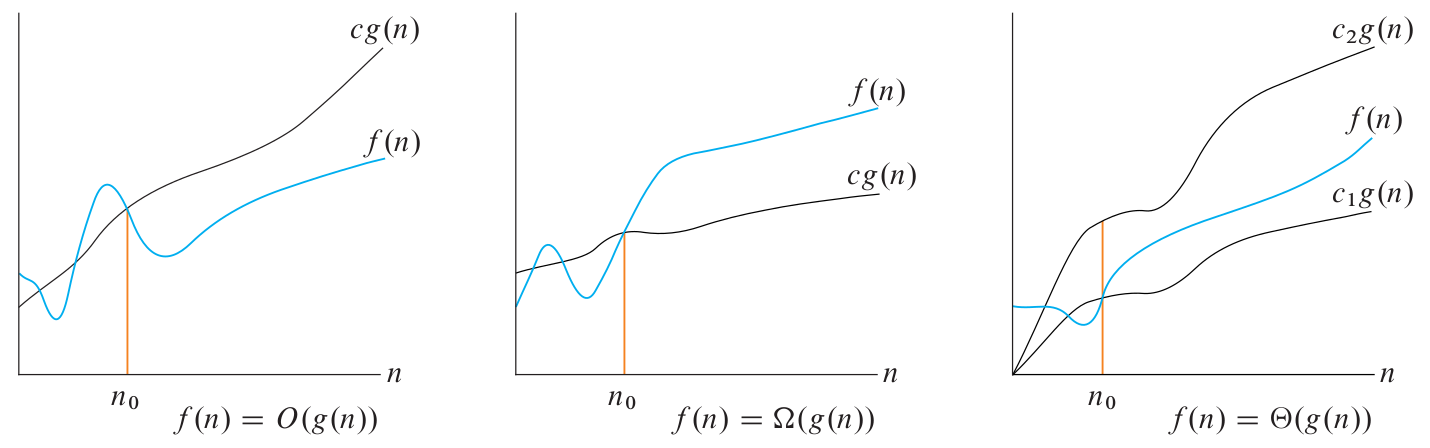
\includegraphics[width=1\textwidth]{figs/chap02/asymptotic}
\end{figure}
\end{itemize}
\end{frame}


\begin{frame}{‌تحلیل مجانبی الگوریتم‌ مرتب‌سازی درجی}
\begin{itemize}\itemr
\item[-]
حال الگوریتم مرتب‌سازی درجی را یک بار دیگر در نظر می‌گیریم.
\begin{algorithm}[H]\alglr
  \caption{Insertion Sort} 
  \begin{algorithmic}[1]
    \Func{Insertion-Sort}{A, n}
    \newline\Comment{A is an array of n elements}
      \For{i = 2 \To n}
        \State key = A[i]
        \State j = i - 1
        \While{ j > 0 and A[j] > key }
          \State A[j+1] = A[j]
          \State j = j-1
        \EndWhile
        \State A[j+1] = key
      \EndFor
  \end{algorithmic}
  \label{alg:insertion-sort}
\end{algorithm}
\end{itemize}
\end{frame}



\begin{frame}{‌تحلیل مجانبی الگوریتم‌ مرتب‌سازی درجی}
\begin{itemize}\itemr
\item[-]
می‌خواهیم اثبات کنیم زمان اجرای این الگوریتم در بدترین حالت
\ath{n^2}
است.
باید اثبات کنیم زمان اجرای الگوریتم 
در بدترین حالت
\m{O(n^2)}
و
\aom{n^2}
است.
\item[-]
این الگوریتم در یک حلقه
\code{for}
به تعداد
\m{n-1}
بار تکرار می‌شود. به ازای هر بار تکرار در این حلقه یک حلقه درونی
\code{while}
وجود دارد که در بدترین حالت
\m{i-1}
بار تکرار می‌شود و i حداکثر n است بنابراین تعداد کل تکرارها در حلقه درونی حداکثر
\m{(n-1)(n-1)}
است، که کران بالای آن
\m{n^2}
 است. بنابراین
\m{T(n) < n^2}
و طبق تعریف کران بالای مجانبی
\m{T(n) = O(n^2)} 
است.
  بنابراین زمان اجرای این الگوریتم
\m{O(n^2)}
است.
\end{itemize}
\end{frame}


\begin{frame}{‌تحلیل مجانبی الگوریتم‌ مرتب‌سازی درجی}
\begin{itemize}\itemr
\item[-]
حال می‌خواهیم نشان دهیم زمان اجرای این الگوریتم در بدترین حالت
\m{\aom{n^2}}
است. برای این کار باید نشان دهیم حداقل یک ورودی وجود دارد که زمان اجرای آن حداقل از مرتبه
\m{n^2}
است.
\item[-]
فرض کنید یکی از ورودی‌های الگوریتم، آرایه‌ای است که طول آن مضرب 
\m{3}
 است و در این ورودی بزرگ‌ترین عناصر آرایه در یک سوم ابتدای آرایه قرار دارند. برای این‌که این آرایه مرتب شود همهٔ این عناصر باید به یک‌سوم انتهای آرایه انتقال پیدا کنند. برای این انتقال هر عنصر باید حداقل
\m{n/3}
بار به سمت راست حرکت کند تا از ثلث میانی آرایه عبور کند. این انتقال باید برای حداقل یک‌سوم عناصر اتفاق بیافتد، پس زمان اجرا در این حالت حداقل
\m{(n/3)(n/3)}
است، بنابراین
\m{T(n) > \frac{1}{9} n^2}
و
 طبق تعریف کران پایین مجانبی
\m{T(n) = \aom{n^2}}
است.
\item[-]
از آنجایی که مرتبه رشد مرتب‌سازی درجی در بدترین حالت حداکثر و حداقل از مرتبه
\m{n^2}
است یعنی مرتبه رشد آن
\m{O(n^2)}
و
\aom{n^2}
است، بنابراین می‌توانیم نتیجه بگیریم مرتبه رشد آن در بدترین حالت از مرتبه
\m{n^2}
است یا به عبارت دیگر
\ath{n^2}
است.
\end{itemize}
\end{frame}